\documentclass[12pt]{article}
\usepackage{amsmath}
\usepackage{graphicx}
\usepackage{hyperref}
\usepackage[utf8]{inputenc}
\usepackage{listings} % For code snippets
\usepackage{tikz} % For UML diagrams
\usetikzlibrary{shapes.geometric, arrows.meta, positioning}
\usepackage{titlesec}
\usepackage{caption}

\title{\Huge Arbitrary Precision Arithmetic Library in Java}
\author{Vansh Gupta \\ CS24BTECH11028}
\date{May 2025}

\begin{document}

\maketitle
    
\section{Introduction}
This report documents the development of an arbitrary-precision arithmetic library in Java for the Software Development Fundamentals (SDF) Project (CS1023). The library supports operations on integers (\texttt{AInteger}) and floating-point numbers (\texttt{AFloat}), handling numbers of any size with up to 30 digits of precision for floating-point division. It includes a command-line interface via \texttt{MyInfArith}.

\section{Structure of my Directory}
\subsection{Class Structure}
The library is organized in the \texttt{arbitraryarithmetic} package with two classes and one class outside with which I am managing:
\begin{itemize}
    \item \texttt{AInteger}: Manages arbitrary-precision integers using an \texttt{ArrayList<Integer>} to store digits.
    \item \texttt{AFloat}: Extends the concept to floating-point numbers, with separate lists of \texttt{intPart} and \texttt{fracPart}.
    \item \texttt{MyInfArith}: Provides a command-line interface to perform operations based on user input.
\end{itemize}

\subsection{UML Class Diagram}
Below is a UML class diagram of the library to have a visual representation of the structure of a system, showing its classes, attributes, methods and the relationships between them.

\begin{figure}[h]
    \centering
    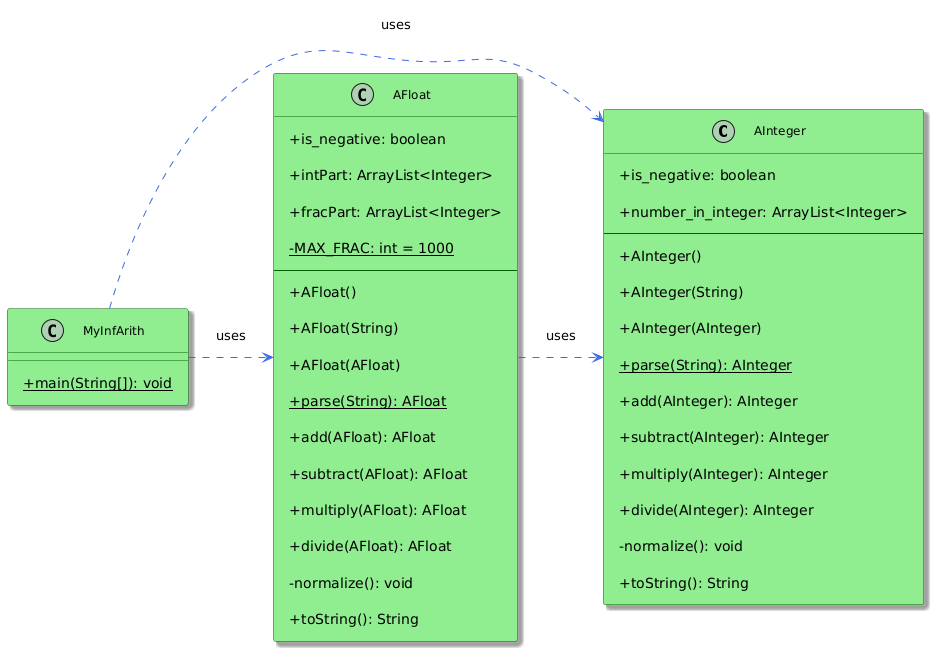
\includegraphics[width=0.9\textwidth]{uml.png}
    \caption*{UML Class Diagram for ArbitraryArithmetic Library}
    \label{fig:uml}
\end{figure}

\subsection{Main Logic}
The arbitrary-precision arithmetic library uses lists to implement addition, subtraction, multiplication, and division. Input strings are converted into digit lists and processed using traditional arithmetic methods. Addition and subtraction iterate through digits, managing carry and borrow in a loop. Multiplication accumulates partial products into a zero-filled array, while division employs repeated subtraction to compute quotient digits iteratively. This list-based approach ensures accurate handling of numbers of any size.

\subsection{Details about Implementation}
\begin{itemize}
    \item \textbf{Storage}: Digits are stored in \texttt{ArrayList<Integer>} to allow unbounded size.
    \item \textbf{Normalization}: Methods like \texttt{normalize()} remove leading/trailing zeros to optimize storage and computation.
    \item \textbf{Addition}: Did addition by using the digit-by-digit method with checking carry in each step and saved the result in the list itself later converted it to string.
    \item \textbf{Subtraction}:Did subtraction by using the digit-by-digit method with checking borrow in each step and saved the result in the list itself later converted it to string.
    \item \textbf{Multiplication}: Did multiplication using a list and saved the result in a list itself later converted it to a string.
    \item \textbf{Division}: \texttt{AFloat.divide} pads the quotient to ensure 30 digits of precision, addressing issues like \texttt{StringIndexOutOfBoundsException} and normal division by using the subtraction method.
\end{itemize}

\section{How to Use the Library}
\subsection{As a Command-Line Tool}
\begin{enumerate}
    \item Compile the project using Ant: \texttt{ant compile}
    \item Create a JAR file: \texttt{ant jar}
    \item To run some test cases: \texttt{ant test}
    \item Run the program with arguments:
    \begin{enumerate}
        \item[\textbf{a.}] \texttt{ant run} or just \texttt{ant} \\
        \hspace*{1em}-- This compiles the program and runs some predefined test cases.
        \item[\textbf{b.}] \texttt{java -jar arbitraryarithmetic/aarithmetic.jar <type> <operation> <num1> <num2>} \\
        \hspace*{1em}-- Runs the program using the generated JAR file.
        \item[\textbf{c.}] \texttt{python3 coderunner.py <type> <operation> <num1> <num2>} \\
        \hspace*{1em}-- Executes the program via the Python script.\\
        \textbf{Note:} Ensure the JAR file exists or create it using \texttt{ant jar}.
        \item[\textbf{d.}] \textbf{Using Docker:}
        \begin{itemize}
            \item Build the Docker image: \\
            \texttt{docker build -t vansh132005/sdfproject .}
            \item Run the container with arguments: \\
            \texttt{docker run vansh132005/sdfproject:latex <type> <operation> <num1> <num2>}
        \end{itemize}
    \end{enumerate}
    \item Example: \texttt{java -jar arbitraryarithmetic/aarithmetic.jar.jar float div 5.5 2}
\end{enumerate}



\subsection{As a Library}
Import the JAR file into your project and use the \texttt{AInteger} and \texttt{AFloat} classes directly.

\section{Limitations}
\begin{itemize}
    \item Floating-point division assumes \texttt{MAX\_FRAC = 30}; higher precision requires adjusting this constant.
    \item Performance may degrade with extremely large numbers due to list-based storage.
    \item No support for advanced mathematical operations (e.g., square root, exponentiation).
\end{itemize}

\section{Verification Approach}
The implementation was tested against the provided public test cases, such as:
\begin{itemize}
    \item \texttt{java MyInfArith float div 5.5 2} $\rightarrow$ \texttt{2.75}
    \item \texttt{java MyInfArith int div 2 0} $\rightarrow$ \texttt{Division by zero error}
\end{itemize}

\section{Key Learnings}
\begin{itemize}
    \item Importance of proper digit management in arbitrary-precision arithmetic.
    \item Handling edge cases like division by zero and precision limits.
    \item Using Ant for build automation simplifies project management.
    \item How to manage such a big project with these many tools and languages such as latex, git and github, ant, docker, python, java, UML.
\end{itemize}

\end{document}